\section{Background}
%Maybe we forego this section and just include them as subsections of Introduction? Or maybe choose a different name.
\subsection{Swarm Robotics}
%Måske skal det her kortes ned og flettes ind i nedenstående punkt?
As mentioned in the introduction, researchers and practitioners in swarm robotics can use a variety of tools to analyze the behavior of robot swarms. This is usually done in one of three ways: Through real robot implementations, computational simulation, or formal verification \parencite{FisherSwarm2010Original}. These different tools for verification and validation each have different advantages and weaknesses. Generally, there exists a trade-off between realism and coverage, and between expresiveness and precision \parencite{VandVpaper}.
\begin{figure}[H]
    \centering
    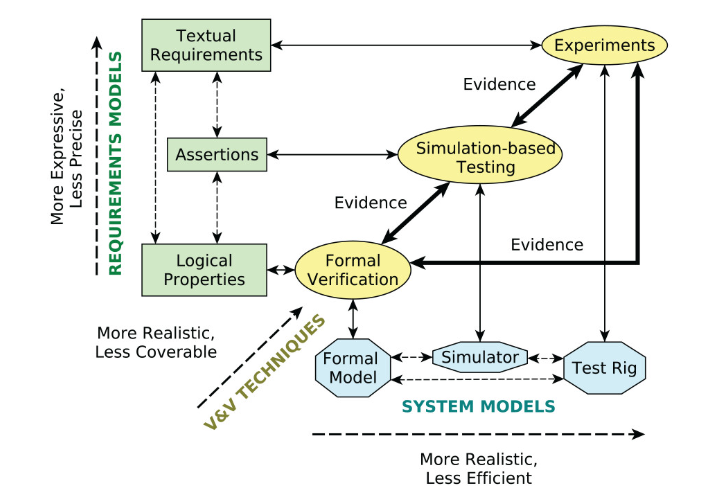
\includegraphics[width=0.8\linewidth]{pictures/FisherFigure.png}
    \caption{An overview of validation and verification (V\&V) techniques. Figure taken from \cite{VandVpaper}.}
    \label{fig:ConsensusGroupsFromArticle}
\end{figure}
%Måske skal det her kortes ned og flettes ind i nedenstående punkt?
In this project, we will be using the modeling tool UPPAAL to model and analyse a swarm robotics algorithm using simulation and statistical model checking. While we aspired to do formal verification as a way to guarantee concrete behaviour of the algorithm, we abandoned this pursuit due to a multitude of reasons. For one, we quickly realized that the state space of our model of the chosen algorithm is very large. This immediately complicates formal verification as the process of exhaustively checking the state space becomes expansive. Secondly, we observed that the interesting, emergent behaviours of our model were not prevalent until larger swarm sizes, further impeding our ability to do relevant formal verification. For these reasons, we elected to pursue model simulations and statistical model checking. We elaborate on this further in section \ref{sec:methodology}.

\subsection{Modeling, verification and properties}

Model checking is a verification technique for assessing* whether a system satisfies properties obtained from its specification \parencite[p. 3]{Baier_Katoen_2008}. Specifically, model checking can be defined as the automated technique of systematically checking whether a given formal property holds for a given finite-state model of a system \parencite[p. 11]{Baier_Katoen_2008}. As can be seen from this definition, model checking involves a number of activities*.* 

First of all, in model checking a \textit{model} is constructed from the system, that is, a formal unambiguous representation of the possible behavior of the given system \parencite[p. 12]{Baier_Katoen_2008}. Whereas the concrete formalism of the model depends on the modelling tool used\footnote{See section 4 for the case of UPPAAL}, the model is usually comprised of a number of states/locations, denoting evaluations of variables etc., and possible transitions between those states, denoting changes in the system (\parencite[p. 12]{Baier_Katoen_2008}). These models are derived from the specification of the system and can be more or less implementation-independent. 

The \textit{properties} to check the system against are also expressed formally in a property specification language, e.g. a linear-temporal logic, expressing propositions about possible behaviour over time, such as "It is always the case that \textit{p} eventually holds" \parencite[p. 12]{Baier_Katoen_2008}.  

Lastly these properties are \textit{checked systematically} on the model. This is done algorithmically by the model checking tool, analysing possible behaviors of the model \parencite[pp. 7, 13]{Baier_Katoen_2008}.

There are a number of motivating factors for using model checking for verification. First, model checking requires stating the system and its specification in formal terms. This encourages that the system under test is understood and expressed unambiguously early on, which can often highlight ambiguities in the specification of the system \parencite[p. 7]{Baier_Katoen_2008}. This has proved useful in our project, as we have found many ambiguities in the specification of the modeled swarm algorithm, many of them early on. We will discuss these later.* 

Another motivation for using model checking is that the system can be modeled and checked against properties at design stage and independent of implementation details. Ideally the model contains only details necessary for property-checking and abstracts away implementation- and hardware specific details. This makes analysis of the system easier, and the model can, afterwards, serve as a guiding blue-print for subsequent (possibly many) implementations of the system \parencite[pp. 145-146]{Brambilla}. This is beneficial in the case of our project, as it makes it possible for us to check properties for the swarm algorithm in a general way before deciding on a specific platform for implementing it.

However, model checking still does not eliminate the potential for errors: The verification is only as good as the model of the system, that is, if the model faithfully represents the system (\cite[pp. 145-146]{Brambilla}, \cite[p. 8]{Baier_Katoen_2008}). As such, we are aware that our model itself can present a source of error, if not done carefully. To account for this, we have made a number of formal properties expressing expected behavior of the system, which the system can be checked against as a sanity check. 


%(evt. lidt om formal verification vs. smc)
%(evt.: lack of fault-injection/faulty systems?)**

%%%Maybe first part should be later in report???***

\subsection{Statistical model checking}
%%Fix citationer!!!
We are using the model-checking tool UPPAAL 5.0 \footnote{\url{https://uppaal.org/}} for modelling and property-checking the swarm algorithm. Especially, we are using features from UPPAAL's statistical model-checker, UPPAAL SMC \footnote{\url{https://uppaal.org/features/}}. Contrary to "classical" UPPAAL, UPPAAL SMC does not \textit{verify} properties as such, by exhausting the entire state space of the model in question. Rather it runs simulations of the system, and uses various statistical results to determine whether a given property is satisfied with a certain degree of confidence \parencite[p. 398]{UPPAALSMC}. This \textit{slacking} of the coverage of model-checking allows utilizing more modelling-features such as floating-point-operations and arbitrary clock-rates*, and it makes model-checking much faster*. As such UPPAAL SMC trades off exhaustive analysis for the feasibility of simulating and checking systems with a much larger state-space. 

%% \textbf{(evt. kort afsnit om model, hvor det viste sig urealistisk at lave symbolsk analyse)***}

We also considered using PRISM\footnote{\url{https://www.prismmodelchecker.org/}} for our model checking. PRISM is a popular tool for modeling systems showing probabilistic behaviour (ref*). But while PRISM also supports statistical model-checking, we found that UPPAAL provided better and more intuitive support for certain modeling features (floating-point-operations, data-structures, functions and initialization of processes*). And in general, we deem the statistical checking features in UPPAAL SMC sufficient for our purpose.

\subsubsection{Basic modelling formalism}

In UPPAAL a system comprises a network of timed automata, each functioning* in parallel \parencite[for a formal definition see:][]{UPPAALTutorial}. A timed automata consists, similar to a finite-state-machine, of a number of locations\footnote{We (as well as UPPAAL) use the term 'location' rather than 'state' as to not conflate it with the state of the automata and the system}*, and a number of edges*. Exactly one of these locations is the \textit{initial} location, meaning that the automaton will always start in that location \url{https://docs.uppaal.org/language-reference/system-description/templates/locations/}. Additionally, an automata can own a number of local variables.  Each edge can have a number of actions (concretely called "updates" in UPPAAL) associated to them, which are performed when enabling the edge, as well a number of guards-conditions required to enable the edge. 

The automaton is \textit{timed} in the sense that it can also contain a number of clocks, the values of which is constrained by invariants on locations. All clocks progresses synchronously and evaluates to a real number at each given moment.* However, individual clocks can be stopped or reset, and alternative clock rates can be specified.*

Automatons can also use globally defined channels for synchronizations. We found that modeling synchronizations through functions rather than channels made our model easier to understand.*

A \textit{state} in a timed automaton is defined by the location, evaluation of its variables and evaluation of its clocks. The state of the entire system is defined by the states of all timed automatons with the addition of evaluations of \textit{globally} defined variables and clocks. A transition, changing the state of the system, can happen in two ways: 1) an automaton enables an edge at a given time, triggering any updates associated with the edge, or 2) an automaton performs a \textit{delay-transition}, staying at it's current location for a given duration $d\in 
\mathds{R}_{+}$, constrained by given invariants. The change is chosen non-deterministically. 

\subsubsection{Making a system in UPPAAL}

In practice, a system made in UPPAAL comprises a number of templates for instantiating timed automatons, global variable declarations, local declarations for instances of each template, and a system declaration for instantiating a number of automatons. An example can be seen in fig \ref{fig:ex-system}, which we will now consider.


\begin{figure}[!b]
    \centering
    \begin{subfigure}{0.90\textwidth}
        \centering
    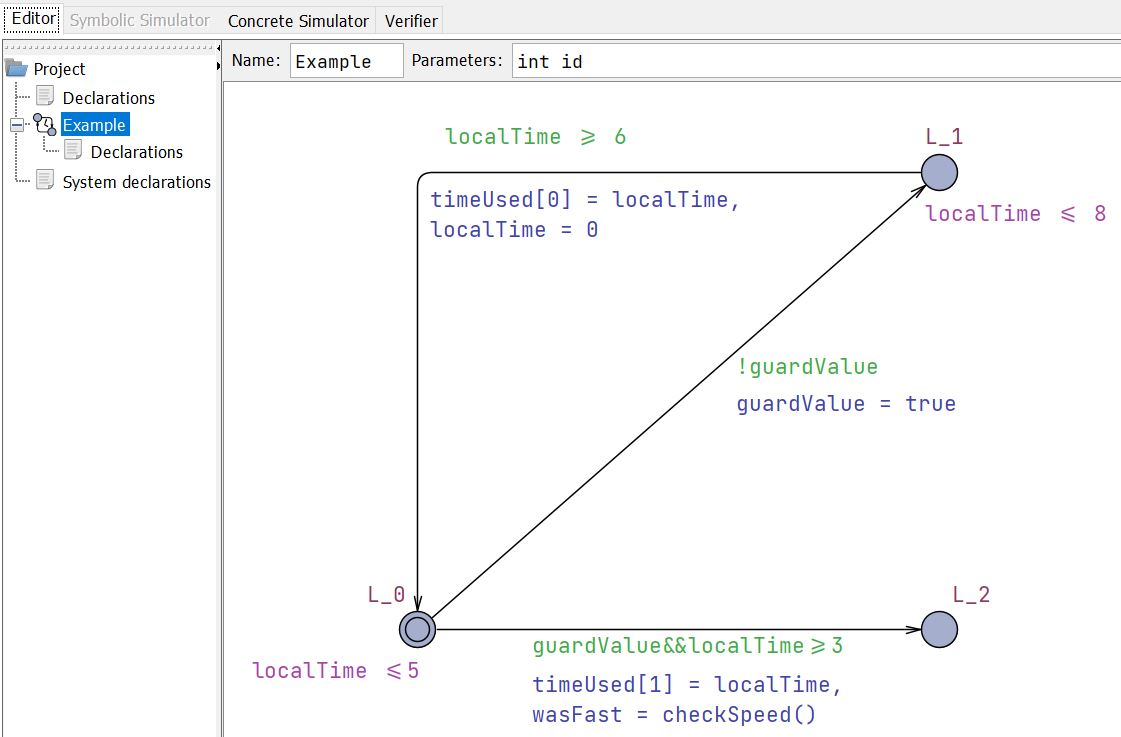
\includegraphics[width=\textwidth]{pictures/example_model_timed.JPG}
    \caption{Template for automata}
    \label{fig:ex-template}
    \end{subfigure}
     
    \medskip
     
    \begin{subfigure}{0.90\textwidth}
         \centering
    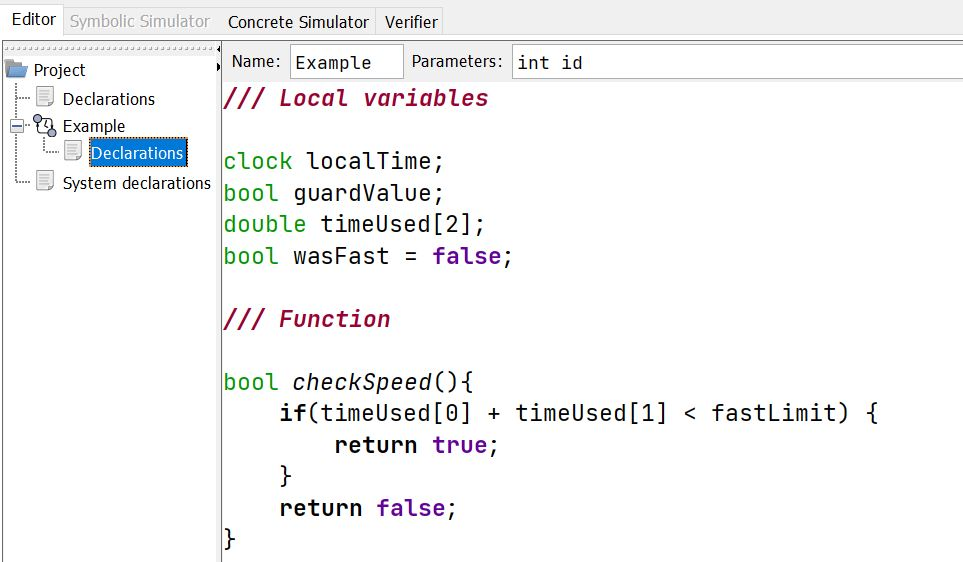
\includegraphics[width=\textwidth]{pictures/Local_declarations_example.JPG}
    \caption{Local declarations}
    \label{fig:ex-local-declarations}
    \end{subfigure}
    
    \caption{Example system in UPPAAL}
\end{figure}

\begin{figure}[ht]\ContinuedFloat
    \centering
    \begin{subfigure}{0.90\textwidth}
         \centering
    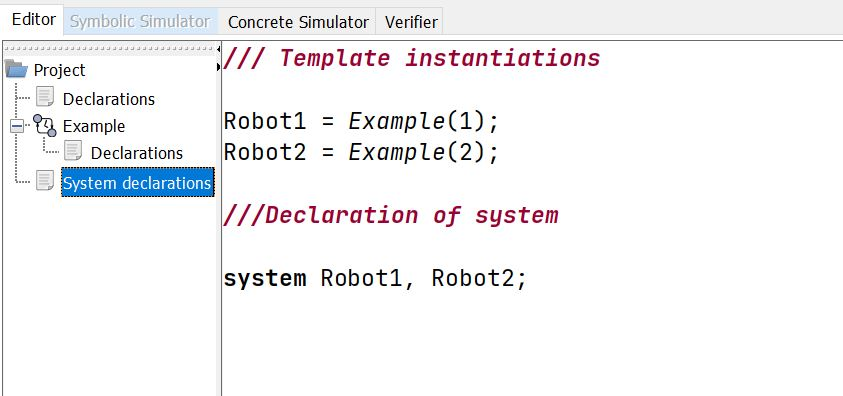
\includegraphics[width=\textwidth]{pictures/System_declaration_example.JPG}
    \caption{System declaration}
    \label{fig:ex-system-declaration}
    \end{subfigure}
     
    \medskip
     
    \begin{subfigure}{0.90\textwidth}
    \centering    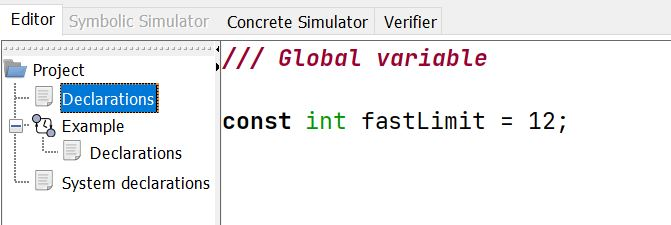
\includegraphics[width=\textwidth]{pictures/global declarations_example.JPG}
    \caption{Global declarations}
    \label{fig:ex-global-declarations}
    \end{subfigure}
    
    \caption{Example system in UPPAAL (cont.)}
    \label{fig:ex-system}
\end{figure}

The global declaration of the system is placed in the "Declarations"-file. In this case (see figure \ref{fig:ex-global-declarations}) the system has just one such value, \verb|fastLimit|, which is a constant of type \verb|int| with value 12.

In this example, the system has just one template, called \verb|Example|. The template has a diagram-representation associated, as seen in fig \ref{fig:ex-template}. Also, indicated in the top, a number of parameters can be specified for the template, specifying arguments that must be given an instantiation of the template \parencite[p. 4]{UPPAALTutorial}. The \verb|Example|-template has just one parameter, \verb|id| of type \verb|int|.

The \verb|Example|-template also has a number of local variables and functions associated to it, as seen in \ref{fig:ex-local-declarations}. In this case, a clock, \verb|localTime|, two boolean values, \verb|guardValue| and \verb|wasFast|, and a size-2-array of type double, \verb|timeUsed[]|. Additionally \verb|Example| has a function, \verb|checkSpeed()|, associated.
%that can be called by \verb|Example|-instances

Looking at the diagram in \ref{fig:ex-system}, the \verb|Example|-template has three locations, denoted by the circles \verb|L_0|, \verb|L_1| and \verb|L_2|. The circle inside \verb|L_0| indicates that it is the initial location of the automaton. At \verb|L_0| and \verb|L_1| invariants are associated, written in purple, indicating bounds on for which interval of values of \verb|localTime| an automaton can be in said state. For example, the automaton can only be in state \verb|L_0| when \verb|localTime| $\in [0,5]$.

There are also a number of edges connecting the locations, indicated by arrows. Each of these edges has a guard associated to it, written in green, and one or more updates, written in blue and separated by ",". For example, the edge from \verb|L_0| to \verb|L_2|
can only be enabled, if \verb|guardValue| evaluates to true and \verb|localTime| exceeds 3. And when the edge is traversed, \verb|timeUsed[1]| is set to the value of \verb|localTime|, after which \verb|wasFast| is set to the value returned by calling \verb|checkSpeed|.
 
Putting all of the above together, an instance of the \verb|Example|-template, goes from \verb|L_0| to \verb|L_1|, back to \verb|L_0| and finally to \verb|L_2| with delays within the time-bound, recording the value of \verb|localTime| at the second and last enabled edge. At the last enabled edge, it is checked, using function \verb|checkSpeed|, whether total time used (stored in \verb|timeUsed|-array) exceeds the global limit \verb|fastLimit|, in which case \verb|wasFast| is set to true. This order of enabling edges is determined by the guards of each edge, which require the first edge to be taken, updating \verb|guardValue| to true, which then makes it possible enabling the edge from \verb|L_0| to \verb|L_2|, but not from \verb|L_0| to \verb|L_1|.

As seen in fig \ref{fig:ex-system-declaration} two instances of the \verb|Example|-template is made with parameters 1 and 2 associated to variables \verb|Robot1| and \verb|Robot2|, after which the system is declared with the \verb|system|-keyword, consisting of the two instances. 

\subsubsection{Statistical model checking}

In UPPAAL SMC these automatons are extended with a stochastic component, replacing non-determinable transitions with probabilistic ones. If a location has a time-invariant, an edge transition is chosen by uniform distribution within that time-constraint. Otherwise one can specify a delay by choosing a rate, $\lambda$ for an exponential distribution for the delay, $d$, with PDF $F(d)=\lambda e^{-\lambda d}$ \parencite[p. 398]{UPPAALSMC}.\footnote{See also: \url{https://docs.uppaal.org/language-reference/system-description/semantics/}} 

When more (possible) edges are present in a given location, a given edge will be enabled according to uniform distribution. Or one can assign each of $n$ edges from a location a given probability, $p_i \in [0,1]$, where $\sum_{i=1}^n p_i = 1 $. 

Applied to our previous example, a modified version of the \verb|Example|-template with this extension could look like \verb|ExampleSMC| in figure \ref{fig:ex-template-smc}.

\begin{figure}[h]
    \centering
    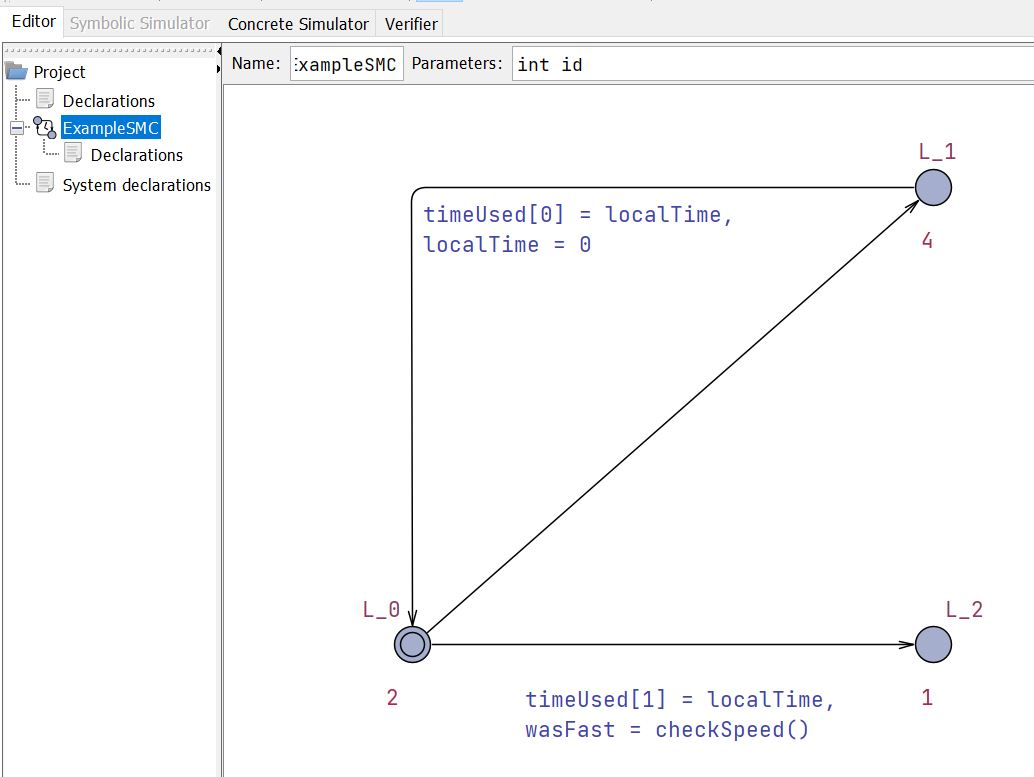
\includegraphics[width=0.90\linewidth]{pictures/example_model_smc.JPG}
    \caption{Example template with stochastic extension}
    \label{fig:ex-template-smc}
\end{figure}

In \verb|ExampleSMC| there are no guards on the edge from \verb|L_0| to \verb|L_1| nor the edge from \verb|L_0| to \verb|L_2|, so one of the edges will be randomly enabled with probability 0.5. Furthermore, instead of invariants, \verb|ExampleSMC| has exponential rates for the PDF of delays in each location, indicated by the brownish integers at each location.

Given this extension, it is possible to perform probabilistic queries on a model. In UPPAAL SMC these are expressed in MITL. These queries take on one of the following forms:

\begin{itemize}
    \item Simulate [\textit{bound}; \textit{N}]\{$expression_1,\, \dotsm \, , expression_n$\}
    \item E[\textit{bound}; \textit{N}]( min $|$ max :  \textit{expression} )
    \item Pr[\textit{bound}]($\phi$)
    \item Pr[\textit{bound}]($\phi$) $\geq$ \textit{probability}
    \item Pr[\textit{bound}$_1$]($\phi_1$) $\geq$ Pr[\textit{bound}$_2$]($\phi_2$)
    
\end{itemize}

Here $\phi$ is an MITL-formula* of the form [ ] $|<>$ \textit{expression}, where [ ] denotes "always holds" and $<>$ denotes "eventually holds".
%%\footnote{UPPAAL also supports full weighted MITL-expressions, but they have not been relevant for us} 
\textit{expression} denotes some state- or variable-based expression. \textit{bound} can be expressed in clock-values or number of edge-transitions.

To answer these queries, UPPAAL runs simulation of random runs of paths bounded by the length of the bounds. In the first two types of queries above, \textit{N} number of those runs are simulated, in which the values of the given expressions are monitored (their evaluation over time in the case of "Simulate"-queries and their expected minimum/maximum value in the case of E-queries). 

As such, if we want to track the value of \verb|localTime| over time in \verb|Robot1| over the course of 100 runs of length less than 10 time-units, we could check the query \verb|simulate [<=10;100]{Robot1.localTime}|. If we instead wanted the average maximum-value of \verb|localTime| for each of those runs, we could have checked the property \verb|E [<=10;100](max : Robot1.localTime)| against the system. 

In the last three cases a variable number of random, bounded runs are simulated, here modelled as Bernoulli random trials, where satisfying the given $\phi$ is equivalent to a success. A number of runs are simulated until, applying smc* algorithms (\cite[see:][]{UPPAALSMC}), the query can be answered with the desired confidence. For example, for checking the query Pr[bound]($\phi$), runs are repeatedly ran until the computed confidence interval has the a decired half-width $\epsilon$ and 
test-coverage $\alpha$.\footnote{\url{https://docs.uppaal.org/language-reference/query-semantics/smc_queries/ci_estimation/}} This mean that the running time of the statistical model checking depends on the desired level of confidence, and is otherwise linear on the bound-length of runs.

For example, if we want to check in the above system,  with confidence $\alpha=0.05$ and half-width $\epsilon=0.05$, the probability that \verb|wasFast| eventually evaluates to true for \verb|Robot1| within 2 time units, we can check the system against the property \verb|Pr[<=2](<>Robot1.wasFast)|. The value of the statistical operators \verb|\alpha| and \verb|\epsilon|, can be set under "Options->Statistical parameters" in the navigation bar. 

\begin{figure}[h]
    \centering
    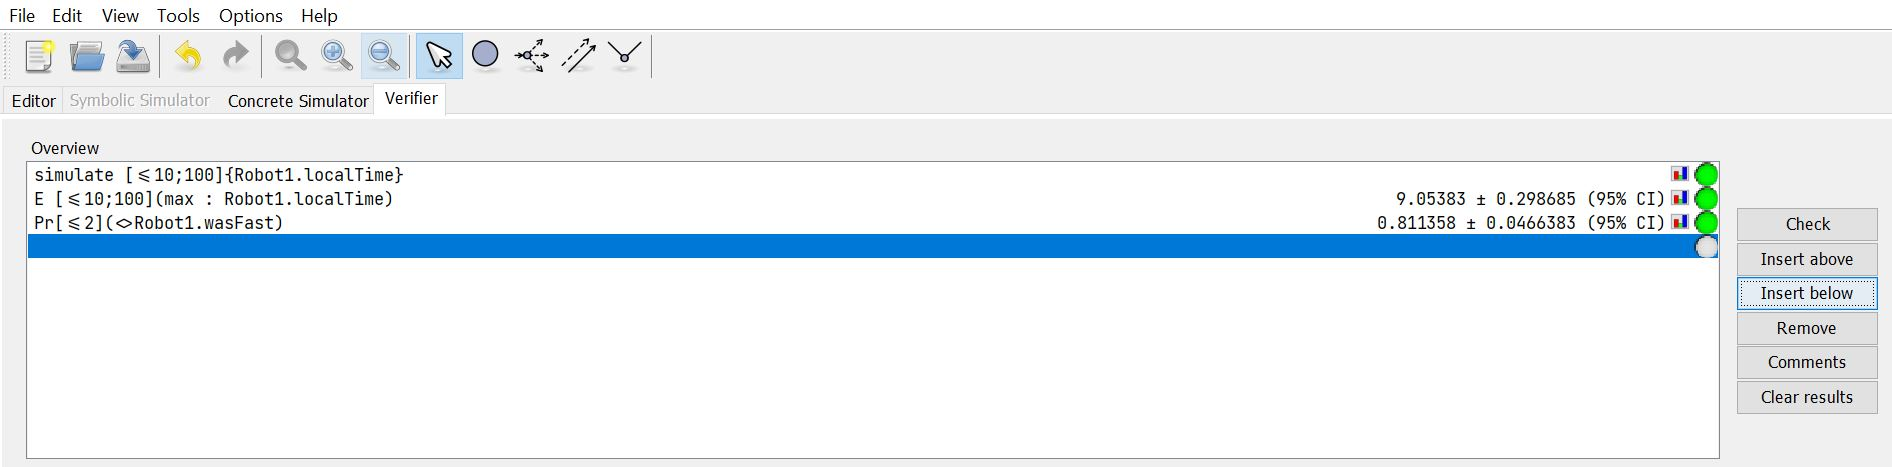
\includegraphics[width=1.0\linewidth]{pictures/properties_example.JPG}
    \caption{Example of probabilistic queries in Uppaal}
    \label{fig:ex-queries}
\end{figure}

As such, rather than exploring the state-space of the model, UPPAAL SMC confines itself to running a number of bounded simulations, which usually result in much faster running times for systems with huge state spaces.\footnote{\url{https://docs.uppaal.org/language-reference/query-semantics/smc_queries/ci_estimation/}}


 